\title{研究タイトル}
\author{プロジェクトマネジメントコース\\
ソフトウェア開発管理グループ\\
矢吹研究室\\
1234567\\
氏名}
\date{}
\begin{document}

\maketitle


 \chapter*{謝辞}

\tableofcontents%目次

 \chapter{序論}
\section{title}
\subsection[タイトル]
\subsubsection{小々節見出し}


 \chapter{背景}
\section{title}
\subsection[タイトル]
\subsubsection{小々節見出し}


\chapter{目的}
\section{title}
\subsection[タイトル]
\subsubsection{小々節見出し}


\chapter{手法}
\section{title}
\subsection[タイトル]
\subsubsection{小々節見出し}


\chapter{結果}
\section{title}
\subsection[タイトル]
\subsubsection{小々節見出し}


\chapter{考察}
\section{title}
\subsection[タイトル]
\subsubsection{小々節見出し}


\chapter{結論}
\section{title}
\subsection[タイトル]
\subsubsection{小々節見出し}


%図の挿入
\begin{figure}[htb]
\centering
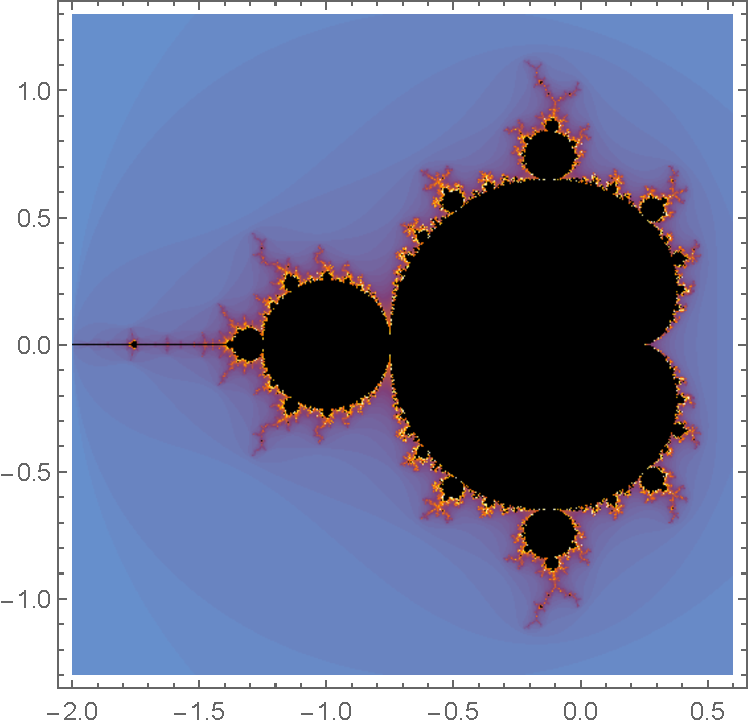
\includegraphics[width=10cm]{figure.pdf}
\caption{図の挿入例}\label{サンプル図}
\end{figure}

参考文献は文献ファイル(この文書では\verb|biblio.bib|)に記述し,\verb|\cite|で参照する.例:データベースのための	問い合わせ言語SQLで数独を解く方法が提案されている\cite{yabuki2011}.このように参照すると,参考文献リストに自動的に登録される.文献の種類には,雑誌論文\cite{yabuki2011}や会議録論文\cite{yabuki2013},卒業論文\cite{kubo2014},書籍\cite{okumura2013},ウェブサイト\cite{self}などがある.文献の種類によって必要な項目が異なるため,\verb|biblio.bib|を見て確認すること.

\bibliographystyle{junsrt}
\bibliography{biblio}%「biblio.bib」というファイルが必要.

\end{document}
